\documentclass[twoside]{book}

% Packages required by doxygen
\usepackage{fixltx2e}
\usepackage{calc}
\usepackage{doxygen}
\usepackage[export]{adjustbox} % also loads graphicx
\usepackage{graphicx}
\usepackage[utf8]{inputenc}
\usepackage{makeidx}
\usepackage{multicol}
\usepackage{multirow}
\PassOptionsToPackage{warn}{textcomp}
\usepackage{textcomp}
\usepackage[nointegrals]{wasysym}
\usepackage[table]{xcolor}

% Font selection
\usepackage[T1]{fontenc}
\usepackage[scaled=.90]{helvet}
\usepackage{courier}
\usepackage{amssymb}
\usepackage{sectsty}
\renewcommand{\familydefault}{\sfdefault}
\allsectionsfont{%
  \fontseries{bc}\selectfont%
  \color{darkgray}%
}
\renewcommand{\DoxyLabelFont}{%
  \fontseries{bc}\selectfont%
  \color{darkgray}%
}
\newcommand{\+}{\discretionary{\mbox{\scriptsize$\hookleftarrow$}}{}{}}

% Page & text layout
\usepackage{geometry}
\geometry{%
  a4paper,%
  top=2.5cm,%
  bottom=2.5cm,%
  left=2.5cm,%
  right=2.5cm%
}
\tolerance=750
\hfuzz=15pt
\hbadness=750
\setlength{\emergencystretch}{15pt}
\setlength{\parindent}{0cm}
\setlength{\parskip}{3ex plus 2ex minus 2ex}
\makeatletter
\renewcommand{\paragraph}{%
  \@startsection{paragraph}{4}{0ex}{-1.0ex}{1.0ex}{%
    \normalfont\normalsize\bfseries\SS@parafont%
  }%
}
\renewcommand{\subparagraph}{%
  \@startsection{subparagraph}{5}{0ex}{-1.0ex}{1.0ex}{%
    \normalfont\normalsize\bfseries\SS@subparafont%
  }%
}
\makeatother

% Headers & footers
\usepackage{fancyhdr}
\pagestyle{fancyplain}
\fancyhead[LE]{\fancyplain{}{\bfseries\thepage}}
\fancyhead[CE]{\fancyplain{}{}}
\fancyhead[RE]{\fancyplain{}{\bfseries\leftmark}}
\fancyhead[LO]{\fancyplain{}{\bfseries\rightmark}}
\fancyhead[CO]{\fancyplain{}{}}
\fancyhead[RO]{\fancyplain{}{\bfseries\thepage}}
\fancyfoot[LE]{\fancyplain{}{}}
\fancyfoot[CE]{\fancyplain{}{}}
\fancyfoot[RE]{\fancyplain{}{\bfseries\scriptsize Generated by Doxygen }}
\fancyfoot[LO]{\fancyplain{}{\bfseries\scriptsize Generated by Doxygen }}
\fancyfoot[CO]{\fancyplain{}{}}
\fancyfoot[RO]{\fancyplain{}{}}
\renewcommand{\footrulewidth}{0.4pt}
\renewcommand{\chaptermark}[1]{%
  \markboth{#1}{}%
}
\renewcommand{\sectionmark}[1]{%
  \markright{\thesection\ #1}%
}

% Indices & bibliography
\usepackage{natbib}
\usepackage[titles]{tocloft}
\setcounter{tocdepth}{3}
\setcounter{secnumdepth}{5}
\makeindex

% Custom commands
\newcommand{\clearemptydoublepage}{%
  \newpage{\pagestyle{empty}\cleardoublepage}%
}

\usepackage{caption}
\captionsetup{labelsep=space,justification=centering,font={bf},singlelinecheck=off,skip=4pt,position=top}

%===== C O N T E N T S =====

\begin{document}

% Titlepage & ToC
\pagenumbering{roman}
\begin{titlepage}
\vspace*{7cm}
\begin{center}%
{\Large Práctica 3 }\\
\vspace*{1cm}
{\large Generated by Doxygen 1.8.11}\\
\end{center}
\end{titlepage}
\clearemptydoublepage
\tableofcontents
\clearemptydoublepage
\pagenumbering{arabic}

%--- Begin generated contents ---
\chapter{Hierarchical Index}
\section{Class Hierarchy}
This inheritance list is sorted roughly, but not completely, alphabetically\+:\begin{DoxyCompactList}
\item \contentsline{section}{Client}{\pageref{class_client}}{}
\item Remote\begin{DoxyCompactList}
\item \contentsline{section}{Client\+\_\+\+Server}{\pageref{interface_client___server}}{}
\begin{DoxyCompactList}
\item \contentsline{section}{Server}{\pageref{class_server}}{}
\end{DoxyCompactList}
\end{DoxyCompactList}
\end{DoxyCompactList}

\chapter{Class Index}
\section{Class List}
Here are the classes, structs, unions and interfaces with brief descriptions\+:\begin{DoxyCompactList}
\item\contentsline{section}{{\bf main} }{\pageref{classmain}}{}
\item\contentsline{section}{{\bf Matrix} \\*\doxyref{Matrix}{p.}{class_matrix} class to create and control a integer matrix.  public }{\pageref{class_matrix}}{}
\end{DoxyCompactList}

\chapter{File Index}
\section{File List}
Here is a list of all files with brief descriptions\+:\begin{DoxyCompactList}
\item\contentsline{section}{C\+:/\+Users/\+Alfredo/workspace/\+P\+\_\+3/src/{\bf A.\+java} }{\pageref{_a_8java}}{}
\item\contentsline{section}{C\+:/\+Users/\+Alfredo/workspace/\+P\+\_\+3/src/{\bf B.\+java} }{\pageref{_b_8java}}{}
\item\contentsline{section}{C\+:/\+Users/\+Alfredo/workspace/\+P\+\_\+3/src/{\bf Contador.\+java} }{\pageref{_contador_8java}}{}
\item\contentsline{section}{C\+:/\+Users/\+Alfredo/workspace/\+P\+\_\+3/src/{\bf main.\+java} }{\pageref{main_8java}}{}
\end{DoxyCompactList}

\chapter{Class Documentation}
\section{A Class Reference}
\label{class_a}\index{A@{A}}
\subsection*{Public Member Functions}
\begin{DoxyCompactItemize}
\item 
synchronized void {\bf Enter\+And\+Wait} ()  throws Interrupted\+Exception
\begin{DoxyCompactList}\small\item\em void \doxyref{Enter\+And\+Wait()}{p.}{class_a_a773d25fe6d1ef55bfe49c0cb809ab5d8}.Prints a message indicating which is the thread that is beginning to run, then it stops for a few seconds , and reprints another message indicating the thread that is running to execute the method all. \end{DoxyCompactList}\end{DoxyCompactItemize}


\subsection{Detailed Description}
public 

\subsection{Member Function Documentation}
\index{A@{A}!Enter\+And\+Wait@{Enter\+And\+Wait}}
\index{Enter\+And\+Wait@{Enter\+And\+Wait}!A@{A}}
\subsubsection[{Enter\+And\+Wait()}]{\setlength{\rightskip}{0pt plus 5cm}synchronized void A.\+Enter\+And\+Wait (
\begin{DoxyParamCaption}
{}
\end{DoxyParamCaption}
) throws Interrupted\+Exception}\label{class_a_a773d25fe6d1ef55bfe49c0cb809ab5d8}


void \doxyref{Enter\+And\+Wait()}{p.}{class_a_a773d25fe6d1ef55bfe49c0cb809ab5d8}.Prints a message indicating which is the thread that is beginning to run, then it stops for a few seconds , and reprints another message indicating the thread that is running to execute the method all. 

\begin{DoxyReturn}{Returns}
void  public synchronized 
\end{DoxyReturn}


The documentation for this class was generated from the following file\+:\begin{DoxyCompactItemize}
\item 
C\+:/\+Users/\+Alfredo/workspace/\+P\+\_\+3/src/{\bf A.\+java}\end{DoxyCompactItemize}

\section{B Class Reference}
\label{class_b}\index{B@{B}}
Inheritance diagram for B\+:\begin{figure}[H]
\begin{center}
\leavevmode
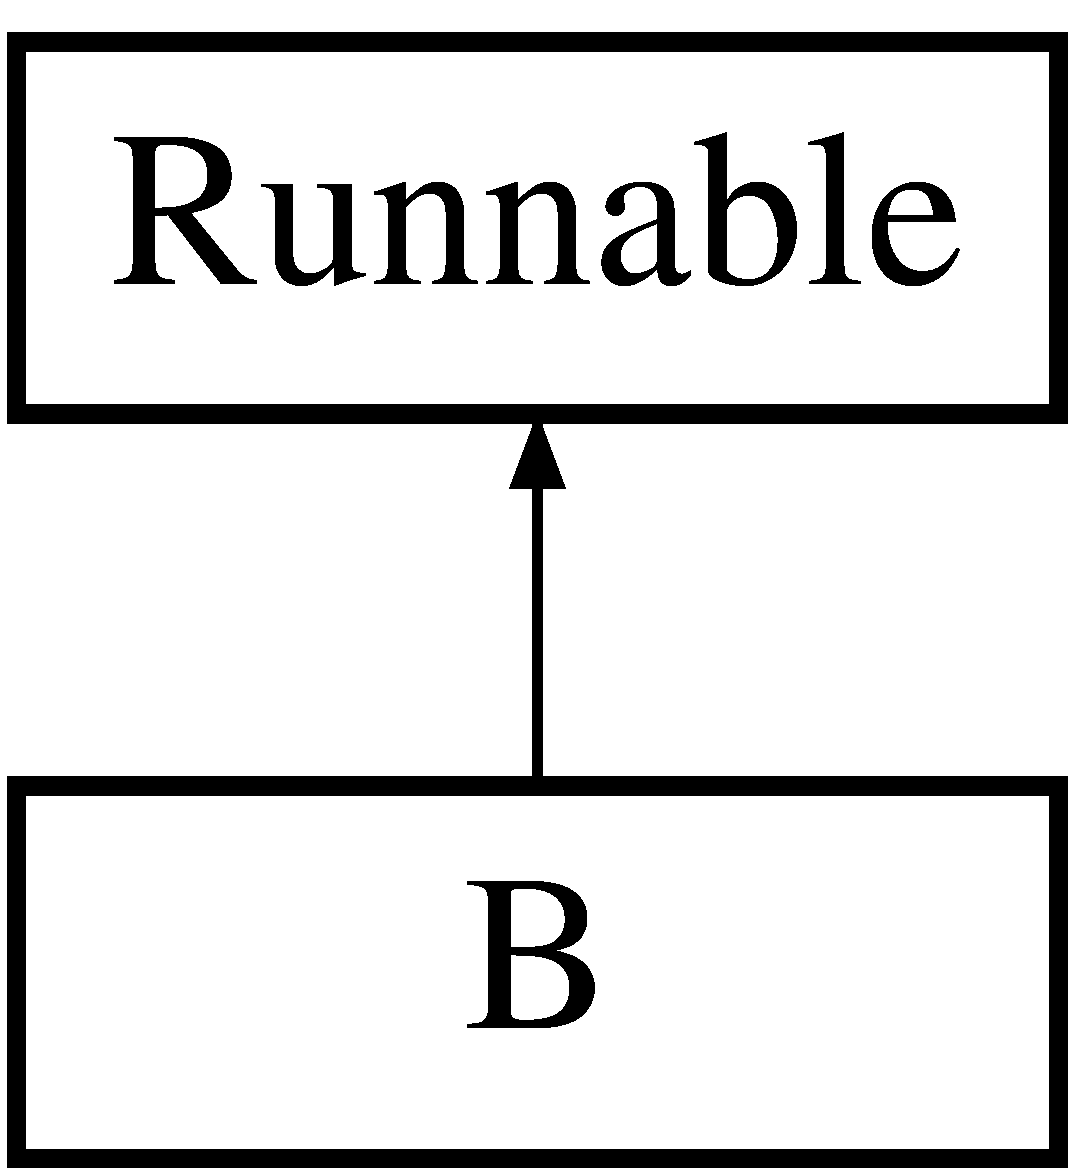
\includegraphics[height=2.000000cm]{class_b}
\end{center}
\end{figure}
\subsection*{Public Member Functions}
\begin{DoxyCompactItemize}
\item 
{\bf B} ({\bf A} object)
\begin{DoxyCompactList}\small\item\em \doxyref{B}{p.}{class_b} constructor. \end{DoxyCompactList}\item 
void {\bf run} ()
\begin{DoxyCompactList}\small\item\em Run function. Running to start the \doxyref{B}{p.}{class_b} object. \end{DoxyCompactList}\end{DoxyCompactItemize}


\subsection{Detailed Description}
public 

\subsection{Constructor \& Destructor Documentation}
\index{B@{B}!B@{B}}
\index{B@{B}!B@{B}}
\subsubsection[{B(\+A object)}]{\setlength{\rightskip}{0pt plus 5cm}B.\+B (
\begin{DoxyParamCaption}
\item[{{\bf A}}]{object}
\end{DoxyParamCaption}
)}\label{class_b_a035f439a504bb428a9c64a2d46ba023e}


\doxyref{B}{p.}{class_b} constructor. 


\begin{DoxyParams}{Parameters}
{\em \doxyref{A}{p.}{class_a}} & object  public \\
\hline
\end{DoxyParams}


\subsection{Member Function Documentation}
\index{B@{B}!run@{run}}
\index{run@{run}!B@{B}}
\subsubsection[{run()}]{\setlength{\rightskip}{0pt plus 5cm}void B.\+run (
\begin{DoxyParamCaption}
{}
\end{DoxyParamCaption}
)}\label{class_b_aba92474eb47bc61bfa0f239a750d090a}


Run function. Running to start the \doxyref{B}{p.}{class_b} object. 

\begin{DoxyReturn}{Returns}
void  public 
\end{DoxyReturn}


The documentation for this class was generated from the following file\+:\begin{DoxyCompactItemize}
\item 
C\+:/\+Users/\+Alfredo/workspace/\+P\+\_\+3/src/{\bf B.\+java}\end{DoxyCompactItemize}

\section{Contador Class Reference}
\label{class_contador}\index{Contador@{Contador}}


Implements a simple concurrent counter.  


Inheritance diagram for Contador\+:\begin{figure}[H]
\begin{center}
\leavevmode
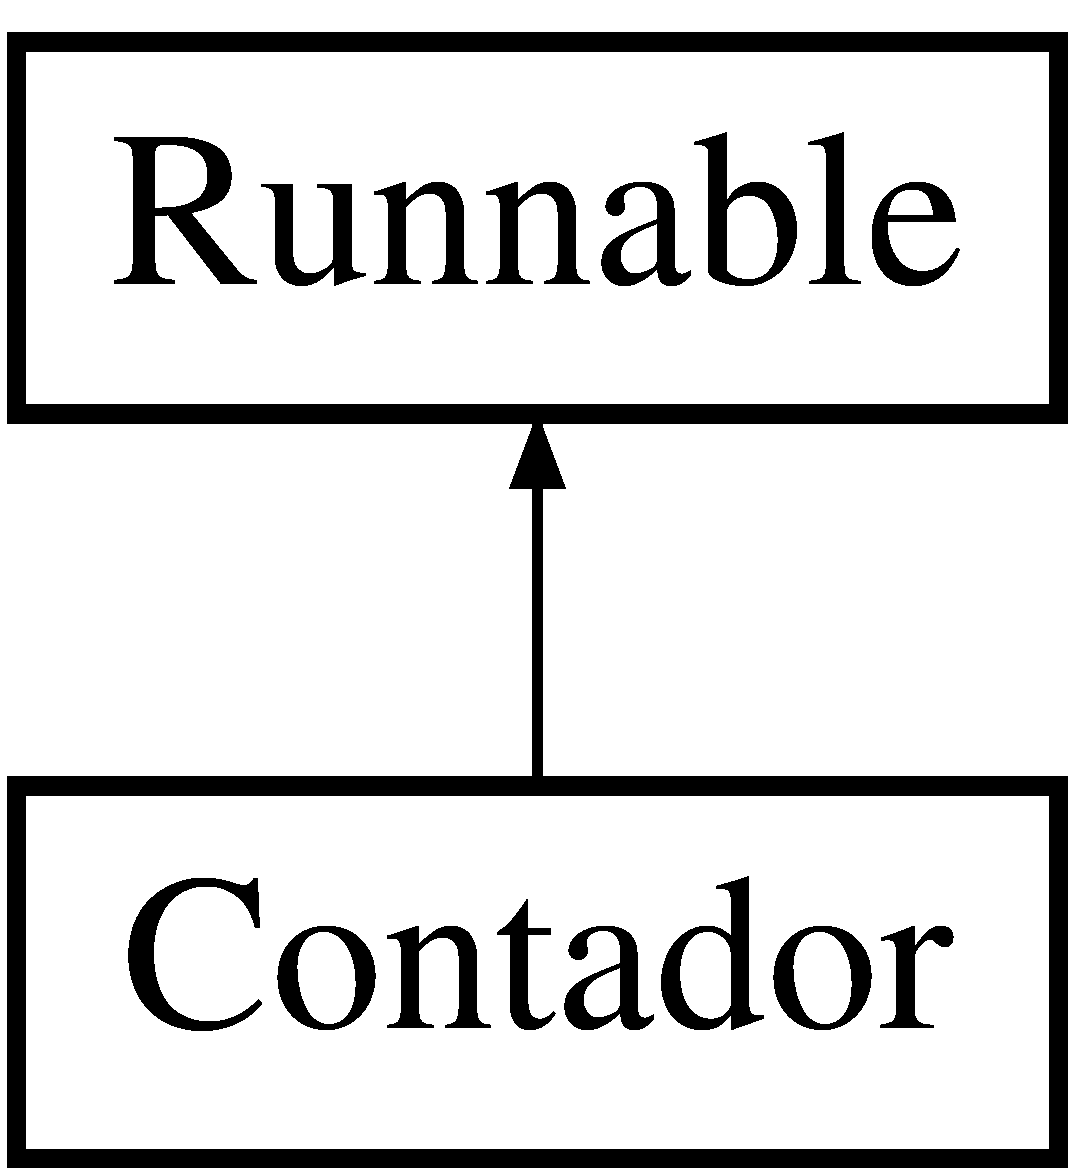
\includegraphics[height=2.000000cm]{class_contador}
\end{center}
\end{figure}
\subsection*{Public Member Functions}
\begin{DoxyCompactItemize}
\item 
synchronized int {\bf incrementar} (int n)
\begin{DoxyCompactList}\small\item\em Executes a loop n iterations that increases an internal variable at a time, and at the end returns current value of that variable. \end{DoxyCompactList}\item 
void {\bf run} ()
\begin{DoxyCompactList}\small\item\em Run function. Running to start the \doxyref{Contador}{p.}{class_contador}. \end{DoxyCompactList}\end{DoxyCompactItemize}


\subsection{Detailed Description}
Implements a simple concurrent counter. 

\subsection{Member Function Documentation}
\index{Contador@{Contador}!incrementar@{incrementar}}
\index{incrementar@{incrementar}!Contador@{Contador}}
\subsubsection[{incrementar(int n)}]{\setlength{\rightskip}{0pt plus 5cm}synchronized int Contador.\+incrementar (
\begin{DoxyParamCaption}
\item[{int}]{n}
\end{DoxyParamCaption}
)}\label{class_contador_a6c069c51fcca68b9056462511c4f2dce}


Executes a loop n iterations that increases an internal variable at a time, and at the end returns current value of that variable. 


\begin{DoxyParams}{Parameters}
{\em int} & n \\
\hline
\end{DoxyParams}
\begin{DoxyReturn}{Returns}
int  public synchronized 
\end{DoxyReturn}
\index{Contador@{Contador}!run@{run}}
\index{run@{run}!Contador@{Contador}}
\subsubsection[{run()}]{\setlength{\rightskip}{0pt plus 5cm}void Contador.\+run (
\begin{DoxyParamCaption}
{}
\end{DoxyParamCaption}
)}\label{class_contador_a09d8777ab2adf697347e960635628071}


Run function. Running to start the \doxyref{Contador}{p.}{class_contador}. 

\begin{DoxyReturn}{Returns}
void  public 
\end{DoxyReturn}


The documentation for this class was generated from the following file\+:\begin{DoxyCompactItemize}
\item 
C\+:/\+Users/\+Alfredo/workspace/\+P\+\_\+3/src/{\bf Contador.\+java}\end{DoxyCompactItemize}

\section{main Class Reference}
\label{classmain}\index{main@{main}}
\subsection*{Static Public Member Functions}
\begin{DoxyCompactItemize}
\item 
static void {\bf main} (String[$\,$] args)  throws Exception 
\begin{DoxyCompactList}\small\item\em Method Main of the project, where other programs are initialized. \end{DoxyCompactList}\end{DoxyCompactItemize}


\subsection{Constructor \& Destructor Documentation}
\index{main@{main}!main@{main}}
\index{main@{main}!main@{main}}
\subsubsection[{main(\+String[] args)}]{\setlength{\rightskip}{0pt plus 5cm}static void main.\+main (
\begin{DoxyParamCaption}
\item[{String[$\,$]}]{args}
\end{DoxyParamCaption}
) throws Exception\hspace{0.3cm}{\ttfamily [static]}}\label{classmain_a0877f3b412d48b8c92fa25c4b98c2f5a}


Method Main of the project, where other programs are initialized. 


\begin{DoxyParams}{Parameters}
{\em args} & \\
\hline
\end{DoxyParams}

\begin{DoxyExceptions}{Exceptions}
{\em Exception} & \\
\hline
\end{DoxyExceptions}
\begin{DoxyReturn}{Returns}
void  public static 
\end{DoxyReturn}


The documentation for this class was generated from the following file\+:\begin{DoxyCompactItemize}
\item 
src/{\bf main.\+java}\end{DoxyCompactItemize}

\chapter{File Documentation}
\section{C\+:/\+Users/\+Alfredo/workspace/\+P\+\_\+3/src/A.java File Reference}
\label{_a_8java}\index{C\+:/\+Users/\+Alfredo/workspace/\+P\+\_\+3/src/\+A.\+java@{C\+:/\+Users/\+Alfredo/workspace/\+P\+\_\+3/src/\+A.\+java}}
\subsection*{Classes}
\begin{DoxyCompactItemize}
\item 
class {\bf A}
\end{DoxyCompactItemize}

\section{C\+:/\+Users/\+Alfredo/workspace/\+P\+\_\+3/src/B.java File Reference}
\label{_b_8java}\index{C\+:/\+Users/\+Alfredo/workspace/\+P\+\_\+3/src/\+B.\+java@{C\+:/\+Users/\+Alfredo/workspace/\+P\+\_\+3/src/\+B.\+java}}
\subsection*{Classes}
\begin{DoxyCompactItemize}
\item 
class {\bf B}
\end{DoxyCompactItemize}

\section{C\+:/\+Users/\+Alfredo/workspace/\+P\+\_\+3/src/\+Contador.java File Reference}
\label{_contador_8java}\index{C\+:/\+Users/\+Alfredo/workspace/\+P\+\_\+3/src/\+Contador.\+java@{C\+:/\+Users/\+Alfredo/workspace/\+P\+\_\+3/src/\+Contador.\+java}}
\subsection*{Classes}
\begin{DoxyCompactItemize}
\item 
class {\bf Contador}
\begin{DoxyCompactList}\small\item\em Implements a simple concurrent counter. \end{DoxyCompactList}\end{DoxyCompactItemize}

\section{C\+:/\+Users/\+Alfredo/workspace/\+P\+\_\+3/src/main.java File Reference}
\label{main_8java}\index{C\+:/\+Users/\+Alfredo/workspace/\+P\+\_\+3/src/main.\+java@{C\+:/\+Users/\+Alfredo/workspace/\+P\+\_\+3/src/main.\+java}}
\subsection*{Classes}
\begin{DoxyCompactItemize}
\item 
class {\bf main}
\end{DoxyCompactItemize}

%--- End generated contents ---

% Index
\backmatter
\newpage
\phantomsection
\clearemptydoublepage
\addcontentsline{toc}{chapter}{Index}
\printindex

\end{document}
